% !TeX root = ../../formal_mordell_weil_rank_2026-07-30.tex
%
% GENERATED FILE -- do not edit by hand.
% Produced by Papers/figures/mordell_weil/make_figures.py
% Okabe--Ito colourblind-safe palette
\definecolor{clrP}{HTML}{0072B2}
\definecolor{clrQ}{HTML}{D55E00}
\definecolor{clrS}{HTML}{009E73}
\definecolor{clrD}{HTML}{CC79A7}
\definecolor{clrBand}{HTML}{56B4E9}
\definecolor{clrGrey}{HTML}{6E6E6E}

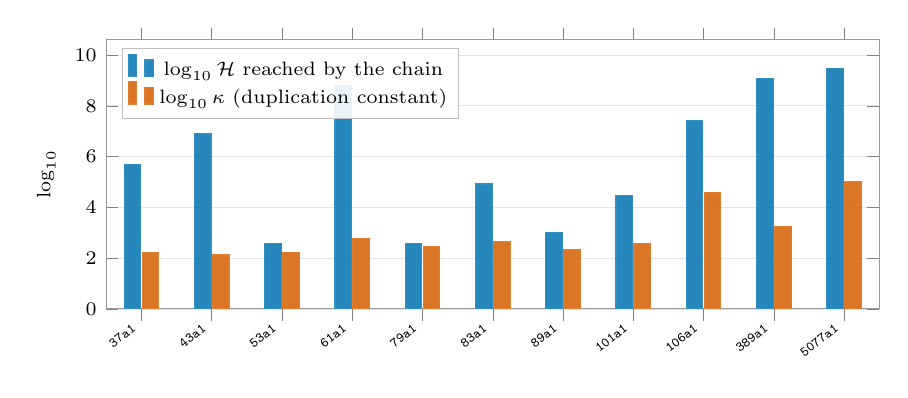
\begin{tikzpicture}
\begin{axis}[
  width=0.94\linewidth, height=5.0cm,
  ybar=0.5pt, bar width=6pt,
  xtick={0,...,10}, xticklabels={\texttt{37a1},\texttt{43a1},\texttt{53a1},\texttt{61a1},\texttt{79a1},\texttt{83a1},\texttt{89a1},\texttt{101a1},\texttt{106a1},\texttt{389a1},\texttt{5077a1}},
  x tick label style={rotate=38, anchor=east, font=\tiny},
  tick label style={font=\scriptsize}, label style={font=\scriptsize},
  ylabel={$\log_{10}$}, ymin=0, ymax=10.6,
  ytick={0,2,4,6,8,10},
  ymajorgrids, grid style={clrGrey!18, line width=0.3pt},
  axis line style={clrGrey!70},
  legend style={font=\scriptsize, at={(0.02,0.97)}, anchor=north west,
                draw=clrGrey!45, fill=white, fill opacity=0.9,
                text opacity=1, row sep=-1.5pt, inner sep=2pt},
  enlarge x limits=0.05,
]
\addplot[fill=clrP, draw=clrP!80, fill opacity=0.85]
  coordinates {(0,5.68134) (1,6.92108) (2,2.56703) (3,8.80400) (4,2.58546) (5,4.92055) (6,3.01030) (7,4.46211) (8,7.42513) (9,9.06787) (10,9.47851)};
\addlegendentry{$\log_{10}\mathcal{H}$ reached by the chain}
\addplot[fill=clrQ, draw=clrQ!80, fill opacity=0.85]
  coordinates {(0,2.23300) (1,2.14301) (2,2.23553) (3,2.77085) (4,2.47422) (5,2.67210) (6,2.34242) (7,2.57171) (8,4.58990) (9,3.23754) (10,5.02430)};
\addlegendentry{$\log_{10}\kappa$ (duplication constant)}
\end{axis}
\end{tikzpicture}
